\newpage
\section{Kết quả và giải thích}
\subsection{Bài 1}
Viết chương trình nhập vào số chấm động. Hãy xuất ra biểu diễn nhị phân từng thành phần (dấu, phần mũ, phần trị) của số chấm động vừa nhập.

\begin{figure}[H]
	\centering
	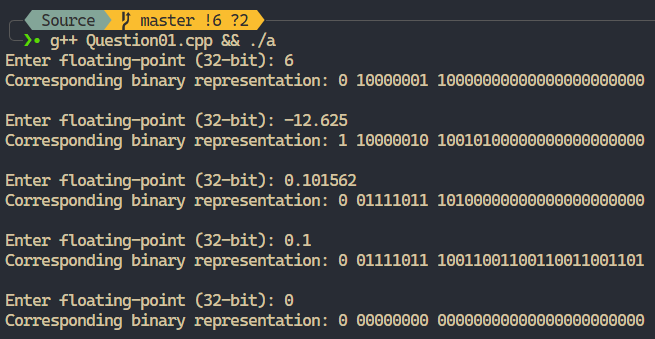
\includegraphics[width=\textwidth]{images/img1.PNG}
	\caption{Chụp màn hình kết quả bài 1.}
\end{figure}

\subsection{Bài 2}

Viết chương trình nhập vào biểu diễn nhị phân của số chấm động. Hãy xuất ra biểu diễn thập
phân tương ứng

\begin{figure}[H]
	\centering
	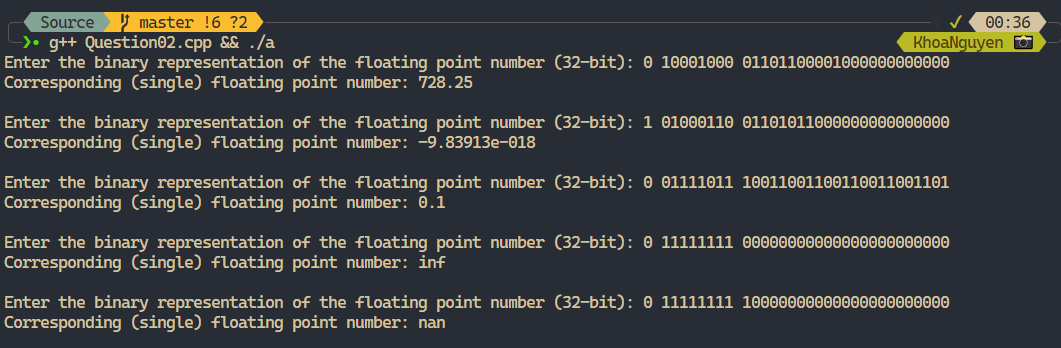
\includegraphics[width=\textwidth]{images/img2.PNG}
	\caption{Chụp màn hình kết quả bài 2.}
\end{figure}

\newpage
\subsection{Bài 3}
Dùng 2 hàm đã viết để khảo sát các câu hỏi:

\begin{itemize}
	\item 1.3E+20 có biểu diễn nhị phân ra sao.
	\item Số float nhỏ nhất lớn hơn 0 là số nào? Biểu diễn nhị phân của nó?
	\item Những trường hợp nào tạo ra các số đặc biệt (kiểu float) (viết chương trình thử nghiệm và giải thích kết quả)
\end{itemize}

\subsubsection{Zero (Số 0)}

Số 0 trong biểu diễn số chấm động có hai dạng: số 0 dương và số 0 âm. Cả hai đều có phần mũ và phần trị bằng 0, chỉ khác nhau ở bit dấu.


\begin{itemize}
	\item Số 0 dương: bit dấu = 0, phần mũ = 0, phần trị = 0.
	\item Số 0 âm: bit dấu = 1, phần mũ = 0, phần trị = 0.
\end{itemize}

Ví dụ, biểu diễn nhị phân của số 0 dương trong chuẩn IEEE 754 (32-bit) là:
\begin{verbatim}
0 00000000 00000000000000000000000
\end{verbatim}

\subsubsection{Denormalized Number (Số không chuẩn hóa)}

Số không chuẩn hóa là các số rất nhỏ gần bằng 0, được sử dụng để biểu diễn các giá trị nhỏ hơn giá trị nhỏ nhất có thể biểu diễn được bằng số chuẩn hóa. Trong biểu diễn số không chuẩn hóa, phần mũ bằng 0 nhưng phần trị khác 0.

\begin{itemize}
	\item Bit dấu: 0 hoặc 1.
	\item Phần mũ: 0.
	\item Phần trị: khác 0.
\end{itemize}

Ví dụ, biểu diễn nhị phân của một số không chuẩn hóa trong chuẩn IEEE 754 (32-bit) là:
\begin{verbatim}
0 00000000 00000000000000000000001
\end{verbatim}

\subsubsection{Infinity (Số vô cùng)}

Số vô cùng được sử dụng để biểu diễn các giá trị vượt quá phạm vi của số chấm động. Có hai dạng: vô cùng dương và vô cùng âm.

\begin{itemize}
	\item Vô cùng dương: bit dấu = 0, phần mũ = 255 (toàn bit 1), phần trị = 0.
	\item Vô cùng âm: bit dấu = 1, phần mũ = 255 (toàn bit 1), phần trị = 0.
\end{itemize}

Ví dụ, biểu diễn nhị phân của số vô cùng dương trong chuẩn IEEE 754 (32-bit) là:
\begin{verbatim}
0 11111111 00000000000000000000000
\end{verbatim}

\subsubsection{NaN (Not a Number - Số không phải là số)}

NaN được sử dụng để biểu diễn các giá trị không hợp lệ hoặc không xác định, chẳng hạn như kết quả của phép chia 0 cho 0 hoặc căn bậc hai của số âm. Có hai loại NaN: NaN yên lặng (quiet NaN) và NaN báo lỗi (signaling NaN).

\begin{itemize}
	\item Bit dấu: 0 hoặc 1.
	\item Phần mũ: 255 (toàn bit 1).
	\item Phần trị: khác 0.
\end{itemize}

Ví dụ, biểu diễn nhị phân của một NaN trong chuẩn IEEE 754 (32-bit) là:
\begin{verbatim}
0 11111111 10000000000000000000000
\end{verbatim}

\subsubsection{X - (+inf)}

Khi thực hiện phép toán `X - (+inf)`, kết quả sẽ là `-inf` (vô cùng âm). Điều này xảy ra vì bất kỳ số hữu hạn nào trừ đi số vô cùng dương đều sẽ dẫn đến kết quả là số vô cùng âm.

\begin{itemize}
	\item Ví dụ: Nếu X = 1.0, thì 1.0 - (+inf) = -inf.
	\item Biểu diễn nhị phân của `-inf` trong chuẩn IEEE 754 (32-bit) là:
	      \begin{verbatim}
1 11111111 00000000000000000000000
\end{verbatim}
\end{itemize}

\subsubsection{(+inf) - (+inf)}

Khi thực hiện phép toán `(+inf) - (+inf)`, kết quả sẽ là `NaN` (Not a Number). Điều này xảy ra vì phép toán này không xác định được giá trị cụ thể, do đó kết quả là một giá trị không phải là số.

\begin{itemize}
	\item Ví dụ: (+inf) - (+inf) = NaN.
	\item Biểu diễn nhị phân của `NaN` trong chuẩn IEEE 754 (32-bit) là:
	      \begin{verbatim}
0 11111111 10000000000000000000000
\end{verbatim}
\end{itemize}

\subsubsection{X / 0}

Khi thực hiện phép toán `X / 0`, kết quả sẽ là `+inf` (vô cùng dương) nếu X là số dương, và `-inf` (vô cùng âm) nếu X là số âm. Điều này xảy ra vì phép chia một số hữu hạn cho 0 dẫn đến kết quả là số vô cùng.

\begin{itemize}
	\item Ví dụ: Nếu X = 1.0, thì 1.0 / 0 = +inf.
	\item Biểu diễn nhị phân của `+inf` trong chuẩn IEEE 754 (32-bit) là:
	      \begin{verbatim}
0 11111111 00000000000000000000000
\end{verbatim}
\end{itemize}

\subsubsection{0 / 0}

Khi thực hiện phép toán `0 / 0`, kết quả sẽ là `NaN` (Not a Number). Điều này xảy ra vì phép toán này không xác định được giá trị cụ thể, do đó kết quả là một giá trị không phải là số.

\begin{itemize}
	\item Ví dụ: 0 / 0 = NaN.
	\item Biểu diễn nhị phân của `NaN` trong chuẩn IEEE 754 (32-bit) là:
	      \begin{verbatim}
0 11111111 10000000000000000000000
\end{verbatim}
\end{itemize}

\subsubsection{(+inf) / (+inf)}

Khi thực hiện phép toán `(+inf) / (+inf)`, kết quả sẽ là `NaN` (Not a Number). Điều này xảy ra vì phép toán này không xác định được giá trị cụ thể, do đó kết quả là một giá trị không phải là số.

\begin{itemize}
	\item Ví dụ: (+inf) / (+inf) = NaN.
	\item Biểu diễn nhị phân của `NaN` trong chuẩn IEEE 754 (32-bit) là:
	      \begin{verbatim}
0 11111111 10000000000000000000000
\end{verbatim}
\end{itemize}

\subsubsection{sqrt(X) với X < 0}

Khi thực hiện phép toán `sqrt(X)` với X < 0, kết quả sẽ là `NaN` (Not a Number). Điều này xảy ra vì căn bậc hai của một số âm không xác định được giá trị cụ thể trong tập số thực, do đó kết quả là một giá trị không phải là số.

\begin{itemize}
	\item Ví dụ: sqrt(-1.0) = NaN.
	\item Biểu diễn nhị phân của `NaN` trong chuẩn IEEE 754 (32-bit) là:
	      \begin{verbatim}
0 11111111 10000000000000000000000
\end{verbatim}
\end{itemize}

\begin{figure}[H]
	\centering
	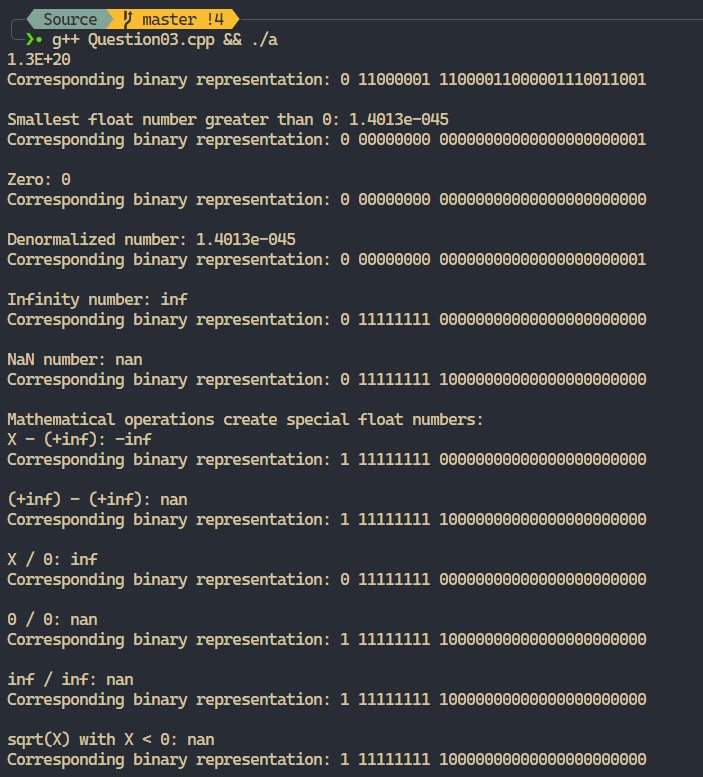
\includegraphics[width=\textwidth]{images/img3.PNG}
	\caption{Chụp màn hình kết quả bài 3.}
\end{figure}

\subsection{Bài 4}
Khảo sát các trường hợp sau đây (viết chương trình thử nghiệm và giải thích kết quả):

\begin{itemize}
	\item Chuyển đổi float -> int -> float.Kết quả như ban đầu ?
	\item Chuyển đổi int -> float -> int. Kết quả như ban đầu ?
	\item Phép cộng số chấm động có tính kết hợp ?
	\item i = (int) (3.14159 * f);
	\item f = f + (float) i;
	\item `if (i == (int)((float) i)) { printf(“true”); }`
	\item if (i == (int)((double) i)) { printf(“true”); }
	\item if (f == (float)((int) f)) { printf(“true”); }
	\item if (f == (double)((int) f)) { printf(“true”); }
\end{itemize}

\subsubsection{Chuyển đổi float -> int -> float. Kết quả như ban đầu?}

Khi chuyển đổi từ `float` sang `int`, phần thập phân của số `float` sẽ bị loại bỏ, chỉ giữ lại phần nguyên. Do đó, khi chuyển đổi ngược lại từ `int` sang `float`, kết quả sẽ không giống như ban đầu nếu số `float` ban đầu có phần thập phân khác 0. Ví dụ, nếu giá trị ban đầu là `3.14159`, sau khi chuyển đổi sang `int` sẽ thành `3`, và khi chuyển đổi ngược lại sang `float` sẽ thành `3.0`. Kết quả này không giống như giá trị ban đầu `3.14159`.

\subsubsection{Chuyển đổi int -> float -> int. Kết quả như ban đầu?}

Khi chuyển đổi từ `int` sang `float`, giá trị của `int` sẽ được giữ nguyên và thêm phần thập phân `.0`. Khi chuyển đổi ngược lại từ `float` sang `int`, phần thập phân sẽ bị loại bỏ, giữ lại phần nguyên. Do đó, kết quả sẽ giống như ban đầu nếu số `float` không có phần thập phân khác 0. Ví dụ, nếu giá trị ban đầu là `42`, sau khi chuyển đổi sang `float` sẽ thành `42.0`, và khi chuyển đổi ngược lại sang `int` sẽ thành `42`. Kết quả này giống như giá trị ban đầu `42`.

\subsubsection{Phép cộng số chấm động có tính kết hợp?}

Phép cộng số chấm động không có tính kết hợp do các vấn đề về độ chính xác và làm tròn trong biểu diễn số chấm động. Ví dụ, với ba số `a = 1.0f`, `b = 1e10f`, và `c = -1e10f`, kết quả của `(a + b) + c` và `a + (b + c)` có thể khác nhau do thứ tự thực hiện phép toán ảnh hưởng đến độ chính xác của kết quả. Trong trường hợp này, `(a + b) + c` có thể cho ra kết quả khác với `a + (b + c)`.

\subsubsection{i = (int) (3.14159 * f);}

Khi thực hiện phép toán `3.14159 * f`, kết quả sẽ là một số `float`. Sau đó, khi chuyển đổi kết quả này sang `int`, phần thập phân sẽ bị loại bỏ, chỉ giữ lại phần nguyên. Ví dụ, nếu `f = 2.0f`, thì `3.14159 * 2.0` sẽ là `6.28318`, và khi chuyển đổi sang `int` sẽ thành `6`.

\subsubsection{f = f + (float) i;}

Khi thực hiện phép toán `f = f + (float) i`, giá trị của `i` sẽ được chuyển đổi sang `float` trước khi thực hiện phép cộng. Ví dụ, nếu `f = 2.0f` và `i = 3`, thì `2.0 + 3.0` sẽ là `5.0`.

\subsubsection{if (i == (int)((float) i)) printf("true");}

Khi thực hiện phép toán `i == (int)((float) i)`, giá trị của `i` sẽ được chuyển đổi sang `float` và sau đó chuyển đổi ngược lại sang `int`. Kết quả sẽ giống như ban đầu nếu giá trị của `i` không có phần thập phân khi chuyển đổi sang `float`. Ví dụ, nếu `i = 3`, thì `3` sẽ được chuyển đổi sang `3.0` và sau đó chuyển đổi ngược lại thành `3`, do đó điều kiện sẽ đúng và in ra `true`.

\subsubsection{if (i == (int)((double) i)) printf("true");}

Khi thực hiện phép toán `i == (int)((double) i)`, giá trị của `i` sẽ được chuyển đổi sang `double` và sau đó chuyển đổi ngược lại sang `int`. Kết quả sẽ giống như ban đầu nếu giá trị của `i` không có phần thập phân khi chuyển đổi sang `double`. Ví dụ, nếu `i = 3`, thì `3` sẽ được chuyển đổi sang `3.0` và sau đó chuyển đổi ngược lại thành `3`, do đó điều kiện sẽ đúng và in ra `true`.

\subsubsection{if (f == (float)((int) f)) printf("true");}

Khi thực hiện phép toán `f == (float)((int) f)`, giá trị của `f` sẽ được chuyển đổi sang `int`, loại bỏ phần thập phân, và sau đó chuyển đổi ngược lại sang `float`. Kết quả sẽ giống như ban đầu nếu giá trị của `f` không có phần thập phân khác 0. Ví dụ, nếu `f = 3.5f`, thì `3.5` sẽ được chuyển đổi sang `3` và sau đó chuyển đổi ngược lại thành `3.0`, do đó điều kiện sẽ sai và in ra `false`.

\subsubsection{if (f == (double)((int) f)) printf("true");}

Khi thực hiện phép toán `f == (double)((int) f)`, giá trị của `f` sẽ được chuyển đổi sang `int`, loại bỏ phần thập phân, và sau đó chuyển đổi ngược lại sang `double`. Kết quả sẽ giống như ban đầu nếu giá trị của `f` không có phần thập phân khác 0. Ví dụ, nếu `f = 3.5f`, thì `3.5` sẽ được chuyển đổi sang `3` và sau đó chuyển đổi ngược lại thành `3.0`, do đó điều kiện sẽ sai và in ra `false`.


\begin{figure}[H]
	\centering
	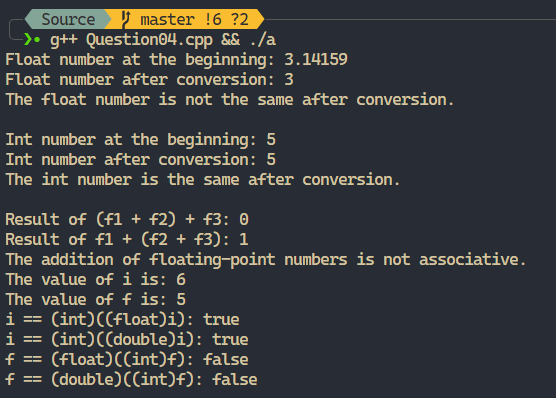
\includegraphics[width=\textwidth]{images/img4.PNG
	}
	\caption{Chụp màn hình kết quả bài 4.}
\end{figure}
